\documentclass{spisok-article}

\title{Робототехнический стенд ``Танчики роботов''}

\author{
	Сергеев Е. Д.,
	студент кафедры системного программирования СПбГУ,
	st040102@student.spbu.ru

	Иванова М.А.,
	студент кафедры системного программирования СПбГУ,
	st040013@student.spbu.ru

	Литвинов Ю.В.,
	доцент кафедры системного программирования СПбГУ, 
	y.litvinov@spbu.ru
}

\begin{document}

\maketitle

\begin{abstract}
В статье представлен новый робототехнический стенд, предназначенный для обучения школьников основам программирования и робототехники, отладки и апробации алгоритмов движения мобильных роботов и группового взаимодействия для студентов. Стенд представляет собой карту с препятствиями, на которой две команды мобильных роботов, вооружённых лазерными излучателями, пытаются ``уничтожить'' друг друга. Статья рассматривает программную часть стенда --- описываются компоненты системы (подсистема коммуникации роботов на базе библиотеки ROS, подсистема определения позиции роботов на карте, интеграция с симулятором V-REP) и реализованные на данный момент алгоритмы.
\end{abstract}

\section{Введение}

Робототехника активно используется в школьной программе для обучения основам информатики и технологии, а также как интересное ученикам направление дополнительного образования, публикуются учебники~(\cite{filippov2017robots, kiselev2017robots}). Чтобы сделать обучение ещё интереснее, проводятся соревнования, существуют целые дисциплины, такие как робофутбол~\cite{luchin2012stand,luchin2012agents}, в соревнованиях участвуют не только школьные, но и студенческие команды. У некоторых соревнований (например, у того же робофутбола) довольно высокий порог вхождения, что затрудняет их применение для обучения школьников и студентов младших курсов, а школьникам остаются простые с алгоритмической точки зрения виды соревнований, такие как различные варианты езды по линии.

Появилась идея создать новую соревновательную дисциплину, где две команды мобильных роботов условно сражаются друг с другом, пытаясь поразить датчики на корпусе робота противника лазерным лучём. Эта задача становится алгоритмически сложной, если команды сражаются в окружении с препятствиями. Чтобы сделать эти соревнования доступными для школьников, потребовалась разработка программно-аппаратного комплекса, который брал бы на себя рутинные (и довольно сложные) задачи коммуникации между роботами, локализации роботов, поиска целей, поиска пути на карте, следования по траектории и низкоуровневого управления устройствами робота~\cite{siegwart2011robots}. Школьникам в таком случае останется решать вопросы стратегии и тактики действий команды, такие как поиск целей на карте, атака цели (возможно, с использованием нескольких роботов), оборона позиции. Таким образом, соревнования сложных алгоритмов могут быть доступными для школьников и достаточно зрелищными, чтобы захватить их интерес.

Реализацию аппаратной части взяли на себя учителя и ученики лицея № 419, программное обеспечение стенда, получившего название ``Танчики роботов'', разрабатывается студентами кафедры системного программирования СПбГУ. В качестве основы для реализации был выбран робототехнический конструктор ТРИК~\cite{terekhov2012trik}, в программной части активно используется ряд проектов с открытым исходным кодом, известных в мире робототехники (не только образовательной, но и профессиональной). Далее в статье описана общая архитектура ПО стенда, то, как в нём применяются третьесторонние компоненты и какие алгоритмы уже реализованы и войдут в стандартную библиотеку.

\section{Концепция и архитектура стенда}

После некоторых исследований в качестве программной платформы для системы управления была выбрана система ROS~\cite{quigley2009ros}. Изначально предполагалось, что команды роботов будут полностью автономны, но от этой концепции пришлось отказаться (возможно, временно) в силу сложности эффективной реализации алгоритмов локализации и построения карты. На данный момент над полем боя находится видеокамера, передающая данные в систему SSL-Vision~\cite{zickler2010sslvision}, широко используемую в робофутболе для локализации роботов команд. SSL-Vision потребовалось модифицировать, чтобы иметь возможность отмечать на карте препятствия и точки интереса. 

Информация о текущих координатах роботов каждой команды, вместе с информацией о координатах препятствий и точек интереса рассылается средствами коммуникации ROS на роботы команд и, при необходимости, на программу, управляющую поведением роботов на симуляторе V-REP~\cite{rohmer2013vrep}. V-REP также может сам выступать в роли средства для получения координат роботов, вместо SSL-Vision, таким образом, симулятор можно использовать параллельно с реальными роботами для визуализации и анализа действий команд, и без реальных роботов вообще, для отладки алгоритмов. На самих роботах (или на симуляторе) находится управляющая программа, пользующаяся библиотекой базовых алгоритмов (например, управления движением) и средой времени выполнения робота TRIK Runtime\footnote{Домашняя страница TRIK Runtime, URL: \url{https://github.com/trikset/trikRuntime} (дата обращения: 24.04.2017г.)}, которая отвечает за работу с аппаратной частью. Структура системы представлена на рисунке~\ref{image:architecture}.

\begin{figure}[ht]
    \centering
    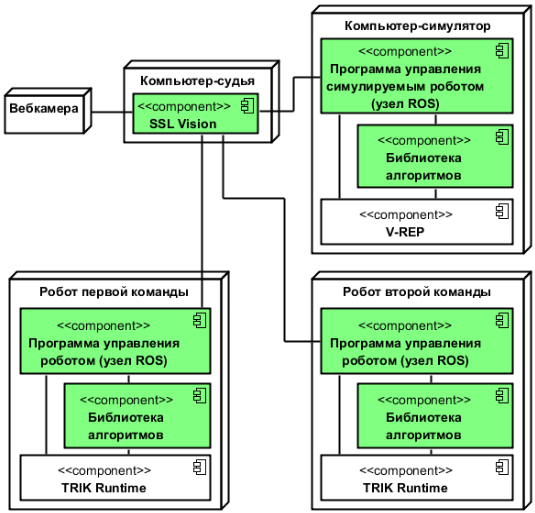
\includegraphics[width=0.8\textwidth]{architecture.png}
    \caption{Архитектура стенда}
    \label{image:architecture}
\end{figure}

Все программные компоненты стенда на данный момент реализованы на языке C++ с использованием библиотеки Qt. Цветом на рисунке~\ref{image:architecture} выделены компоненты, которые потребовалось разработать или модифицировать в рамках проекта.

\section{Использование ROS}

ROS (Robot Operating System)~\cite{quigley2009ros} --- Операционная система для роботов --- это фреймворк для программирования роботов, предоставляющий функциональность для распределённой работы, имеющий множество готовых компонент. ROS обеспечивает разработчиков библиотеками и инструментами для создания приложений робототехники. ROS обеспечивает аппаратную абстракцию, предлагает драйверы устройств, библиотеки, визуализаторы, обмен сообщениями, менеджеры пакетов и многое другое. ROS выпускается в соответствии с условиями лицензии BSD и с открытым исходным кодом.

С точки зрения архитектуры ROS представляет собой распределенную вычислительную систему, состоящую из множества независимых узлов, которые могут быть запущены на различных физических устройствах под управлением разных операционных систем, обменивающихся сообщениями с использованием TCP или UDP, используя модель издатель-подписчик, путем публикации сообщений и подписки на них (топики), либо путем удаленных вызовов (сервисы).

С точки зрения функциональности фреймворк ROS можно разделить на пакеты, предоставляющие возможности по взаимодействию с другими узлами, и пакеты, реализующие различные алгоритмы, использующие данные, производимые другими пакетами.

Связь между узлами сети осуществляется с помощью мастер-узла, который регистрирует запущенные узлы и предоставляет информацию о топиках и сервисах. Перед началом публикации сообщений в канал каждый узел сообщает об этом мастер-узлу, для получения сообщений узлы подписываются на каналы. Узлы используют мастер-узел только для того, чтобы узнать адреса друг друга, обмениваются сообщениями они друг с другом напрямую.  ROS предоставляет клиентские библиотеки для реализации узлов на различных языках программирования.

В системе ROS на стенде находятся команды роботов, сервер с SSL-Vision и, при необходимости, компьютеры судей. Роботы обмениваются друг с другом сообщениями внутри своих команд и получают сообщения от SSL-Vision с координатами других роботов своей команды.

\section{Интеграция с SSL-Vision}

SSL-Vision (The Shared Vision System for the RoboCup Small Size League)~\cite{zickler2010sslvision} является системой зрения, разделяемой несколькими командами роботов. Система обрабатывает в режиме реального времени изображения, снимаемые несколькими камерами, расположенными над полем. SSL-Vision определяет местоположения роботов, а затем передает каждому роботу координаты других роботов его команды. Определение команды робота происходит на основе его ``шапки'' --- разноцветного изображения, расположенного сверху на роботе, уникального для команды в рамках данной сессии.

В рамках работы был написан плагин для SSL-Vision, который позволяет судьям отмечать на статическом изображении неподвижные объекты (стены, препятствия, лабиринт и т.д.) в качестве списка пар точек, а затем посредством TCP отправлять местоположения этих объектов всем роботам в системе ROS. Также возможно отмечать точки на карте, что может быть полезно для отработки командных алгоритмов. Архитектура плагина спроектирована таким образом, что при добавлении возможности отмечать объекты новых типов, отличающихся от отрезков и точек, не придется изменять основную логику плагина.

SSl-Vision, а также вышеупомянутый плагин, работают как два различных узла в системе ROS, и отправляют сообщения, предварительно сериализованные в формате protobuf\footnote{Широко используемый формат передачи данных, URL: \url{https://github.com/google/protobuf} (дата обращения: 24.04.2017г)}, в соответствующие топики.

\section{Интеграция с V-REP}

V-REP~\cite{rohmer2013vrep} --- робосимулятор с интегрированной средой разработки, основанный на распределенной архитектуре управления: каждый объект/модель может управляться индивидуально с помощью встроенного сценария, плагина, узла ROS, клиента удаленного API.

На нашем стенде каждый робот представляет собой отдельный узел, поэтому мы начали разработку библиотеки, позволяющей управлять роботами, находящимися на сцене V-REP, с помощью ROS узлов.

Для того чтобы узлы могли коммуницировать, необходимо запустить roscore - ядро ROS, которое состоит из мастер-узла, потоков ввода/вывода и сервера параметров, который используется узлами для хранения и извлечения параметров во время работы. Задача roscore это поиск и соединение работающих узлов ROS. В случае такого управления V-REP должен выступать в качестве узла ROS, тогда  другие узлы, находящиеся на сцене, смогут общаться через сервисы, издателей и подписчиков ROS. V-REP поддерживает два способа управления через ROS:  rosPlugin и RosInterface. В нашей реализации использовался второй подход, т.к. RosInterface поддерживает больше функций для управления сценой, объектами и моделями, и дублирует API C/C++, в отличие от RosPlugin, который является более старой версией и представляет собой более высокий уровень абстракции. Функциональность RosInterface включена через плагины, код которых является открытым и может быть адаптирован к необходимым потребностям. Плагины загружаются при запуске V-REP, но операция загрузки будет успешна  только в том случае, когда запущен roscore.

Для того чтобы управление моделями на сцене происходило через узел ROS, необходимо запустить управляющую программу из V-REP, для этого следует закрепить за объектом или моделью на сцене V-REP скрипт, который представляет собой код на языке Lua. В нем, с помощью стандартных функций V-REP можно вызвать нужный бинарный файл.  Также в этом скрипте необходимо инициализировать подписчиков и издателей для получения и отправки сообщений.

Запущенный в V-REP исполняемый файл должен инициализировать ROS, создавать узел и после этого подписчиков, которые будут получать сообщения от издателей, инициализированных в V-REP, и издателей, отправляющих сообщения узлам V-REP, которые подписаны на них.

\section{Реализованные алгоритмы}

Окружающая среда реального робота сильно влияет на его поведение, поэтому для отладки алгоритмов движения использовался симулятор V-REP. В качестве робота была выбрана трехколесная модель с двумя управляющими колесами и одним --- поддерживающим. В управляемые колеса  были добавлены динамические суставы, которые выполняют движение вместе с колесом. Функции V-REP позволяют получить в радианах угол поворота такого сустава, который изменяется в диапазоне $[-pi, pi]$, и с помощью функциональности ROS полученные данные можно передать в метод, написанный на языке C++, и далее его обработать. 

Для того, чтобы робот мог выполнять движения, используя энкодеры, был реализован метод, в котором вычисление числа отсчетов энкодера производится по формуле:
\[encVal = \left\{
  \begin{array}{lr}
    \frac{val}{2 * pi} + stepEncoder,             & val \ge 0 \\
    \frac{2 * pi - |val|}{2 * pi} + stepEncoder,  & val < 0
  \end{array}
\right.
\]
где $val$ --- значение угла в радианах, полученное от издателя из V-REP, и $stepEncoder$ --- количество полных оборотов колеса, $encVal$ --- значение энкодера. Пройденное расстояние вычисляется по формуле
$$distance = encVal * pi * R$$
где $R$ --- радиус колеса.

Выбранная модель робота в V-REP схожа с моделью трехколесной тележки, собранной из робототехнического конструктора ТРИК.  Для реальной модели были проведены исследования работы энкодеров, а именно, было реализовано два способа, позволяющих вычислить пройденное расстояние роботом. В первом измерения проводились лишь по датчику одного из колес, и расстояние рассчитывается по формуле:
$$dist = 2 * pi * R * \frac{turn}{configTurn}$$
где $dist$ --- итоговое расстояние, $turn$ --- количество отсчетов энкодеров полученных с датчика, $configTurn$ --- количество отсчетов энкодеров за один оборот колеса, $R$ --- радиус колеса.

Во втором способе использовались показания обоих датчиков и использовались формулы:
$$turn = \frac{turn_1 + turn_2}{2}$$
$$dist = 2 * pi * R * \frac{turn}{configTurn}$$
где $dist$ --- итоговое расстояние, $turn$ --- количество отсчетов энкодеров, равное среднему арифметическому значений, полученных с датчика, $configTurn$ --- количество энкодеров за один оборот колеса, $R$ --- радиус колеса.

\section{Заключение}

В работе была описана программная часть робототехнического стенда ``Танчики роботов''. Стенд всё ещё находится в стадии активной разработки, библиотека алгоритмов и доступный инструментарий продолжают расширяться\footnote{Исходные коды проекта доступны по ссылке \url{https://github.com/yurii-litvinov/TrikABCL} (дата обращения: 23.04.2017г).}. Наиболее важным направлением будущей работы является создание визуального языка для программирования действий команд роботов в среде TRIK Studio [ссылки, тысячи их], что сделает работу со стендом доступной даже для людей, вообще не умеющих программировать. Также важным этапом будет апробация представленных инструментов при проведении реального соревнования, что планируется сделать осенью 2017 года.

\renewcommand\refname{Литература}
\begin{thebibliography}{8}
	\bibitem{filippov2017robots} Филиппов С. А. Уроки робототехники. Конструкция. Движение. Управление. -- Лаборатория знаний, 2017. -- 176 C.
	\bibitem{kiselev2017robots} М. М. Киселев, М. М. Киселев. Робототехника в примерах и задачах. Курс программирования механизмов и роботов. -- Солон-Пресс, 2017. -- 136 С.
	\bibitem{luchin2012stand} Р.М. Лучин, И.Ю. Широколобов, Учебно-исследовательский стенд для мультиагентных систем управления комплексами динамических объектов // Материалы конференции ``Информационные технологии в управлении'' (ИТУ-2012), С. 858-860.
	\bibitem{luchin2012agents} Р.М. Лучин, И.Ю. Широколобов, К.С. Овчинников, Г.П. Облапенко. Исследование алгоритмов мультиагентного взаимодействия с помощью робототехнического комплекса // Материалы конференции ``Информационные технологии в управлении'' (ИТУ-2012), С. 213-215.
	\bibitem{siegwart2011robots} R. Siegwart, I. R. Nourbakhsh, D. Scaramuzza. Introduction to autonomous mobile robots. -- MIT press, 2011. -- 472 pp.
	\bibitem{terekhov2012trik} A.N. Terekhov, R.M. Luchin, S.A. Filippov. Educational cybernetical construction set for schools and universities // IFAC Proceedings Volumes (IFAC-PapersOnline), 9 (PART 1). -- 2012. -- pp. 430-435
	\bibitem{quigley2009ros} M. Quigley et al. ``ROS: An open-source robot operating system,'' // in Proc. ICRA Open-Source Softw. Workshop, 2009.
	\bibitem{zickler2010sslvision} S. Zickler et al. SSL-vision: The shared vision system for the RoboCup Small Size League. // Robo Cup 2009: Robot Soccer World Cup XIII. -- 2010. -- pp. 425–436
	\bibitem{rohmer2013vrep} E. Rohmer, S. P. N. Singh, M. Freese. V-REP: A versatile and scalable robot simulation framework // 2013 IEEE/RSJ International Conference on Intelligent Robots and Systems.
\end{thebibliography}

\end{document}
